\documentclass{article}
\author{Pedro de Carvalho Braga Ilidio Silva - 9762595}
\title{Projeto 4 — Movimento realístico}
\date{19 de maio de 2017}

\usepackage[utf8]{inputenc}
\usepackage{graphicx}
\usepackage{listings}
\usepackage{amsmath}
\usepackage[a4paper, total={19cm, 27cm}]{geometry}

\begin{document}
\maketitle
\section{Introdução}

\section{Efeito resistivo do ar em bicicletas}

Partir-se-á da seguinte equação, que se trata de uma aproximação numérica para a velocidade \(v\) do centro de massa de um objeto em movimento retilíneo (bicicleta), obtida por meio do método de Euler.

\begin{equation}
  \label{eq:vel}
  v_{i+1} = v_i + \frac{P}{mv_i} \Delta t -\frac{\rho Av^2_i}{2m} \Delta t
\end{equation}

É facilmente perceptível, pela equação \ref{eq:vel}, a inviabilidade de se aplicar este método a movimentos posteriores a instantes de repouso, em que a velocidade é nula, pois deparar-se-ia com divisão por zero no segundo termo e não seria possível dar continuidade aos procedimetos recursivos.\par
Foram definidos os seguintes termos como constantes:

\begin{itemize}
\item Massa: \(m = 70 kg\)
\item Potência: \(P = 400 W\)
\item Duração do movimento, máximo instante considerado: \(t_{max}=300 s\)
\item Intervalo entre os instantes de tempo considerados: \(\Delta t = 0.1s\)
\item Velocidade inicial: \(v_0 = 4 m/s\)
\item Densidade do ar: \(\rho\)
\item Area frontal do objeto: \(A\)
\end{itemize}
A partir dos quais foi elaborado um programa em Fortran90 para estimar a velocidade da bicicleta nos instantes determinados pelos parâmetros. Tal programa se baseava em um laço DO, que reatribuia um novo valor de velocidade a uma variável V em cada ciclo, de acordo com a \ref{eq:1}.

Os valores para o caso em que \(\rho =0\) foram então coletados em arquivo e graficados (Gráfico 1). No mesmo gráfico são também apresentados os valores exatos da velocidade, determinados pela equação \ref{eq:2}. 

\begin{equation}
  \label{eq:2}
  v(t) = v^2_0 + {2Pt \over m}
\end{equation}

\begin{figure}[h!]
  \centering
  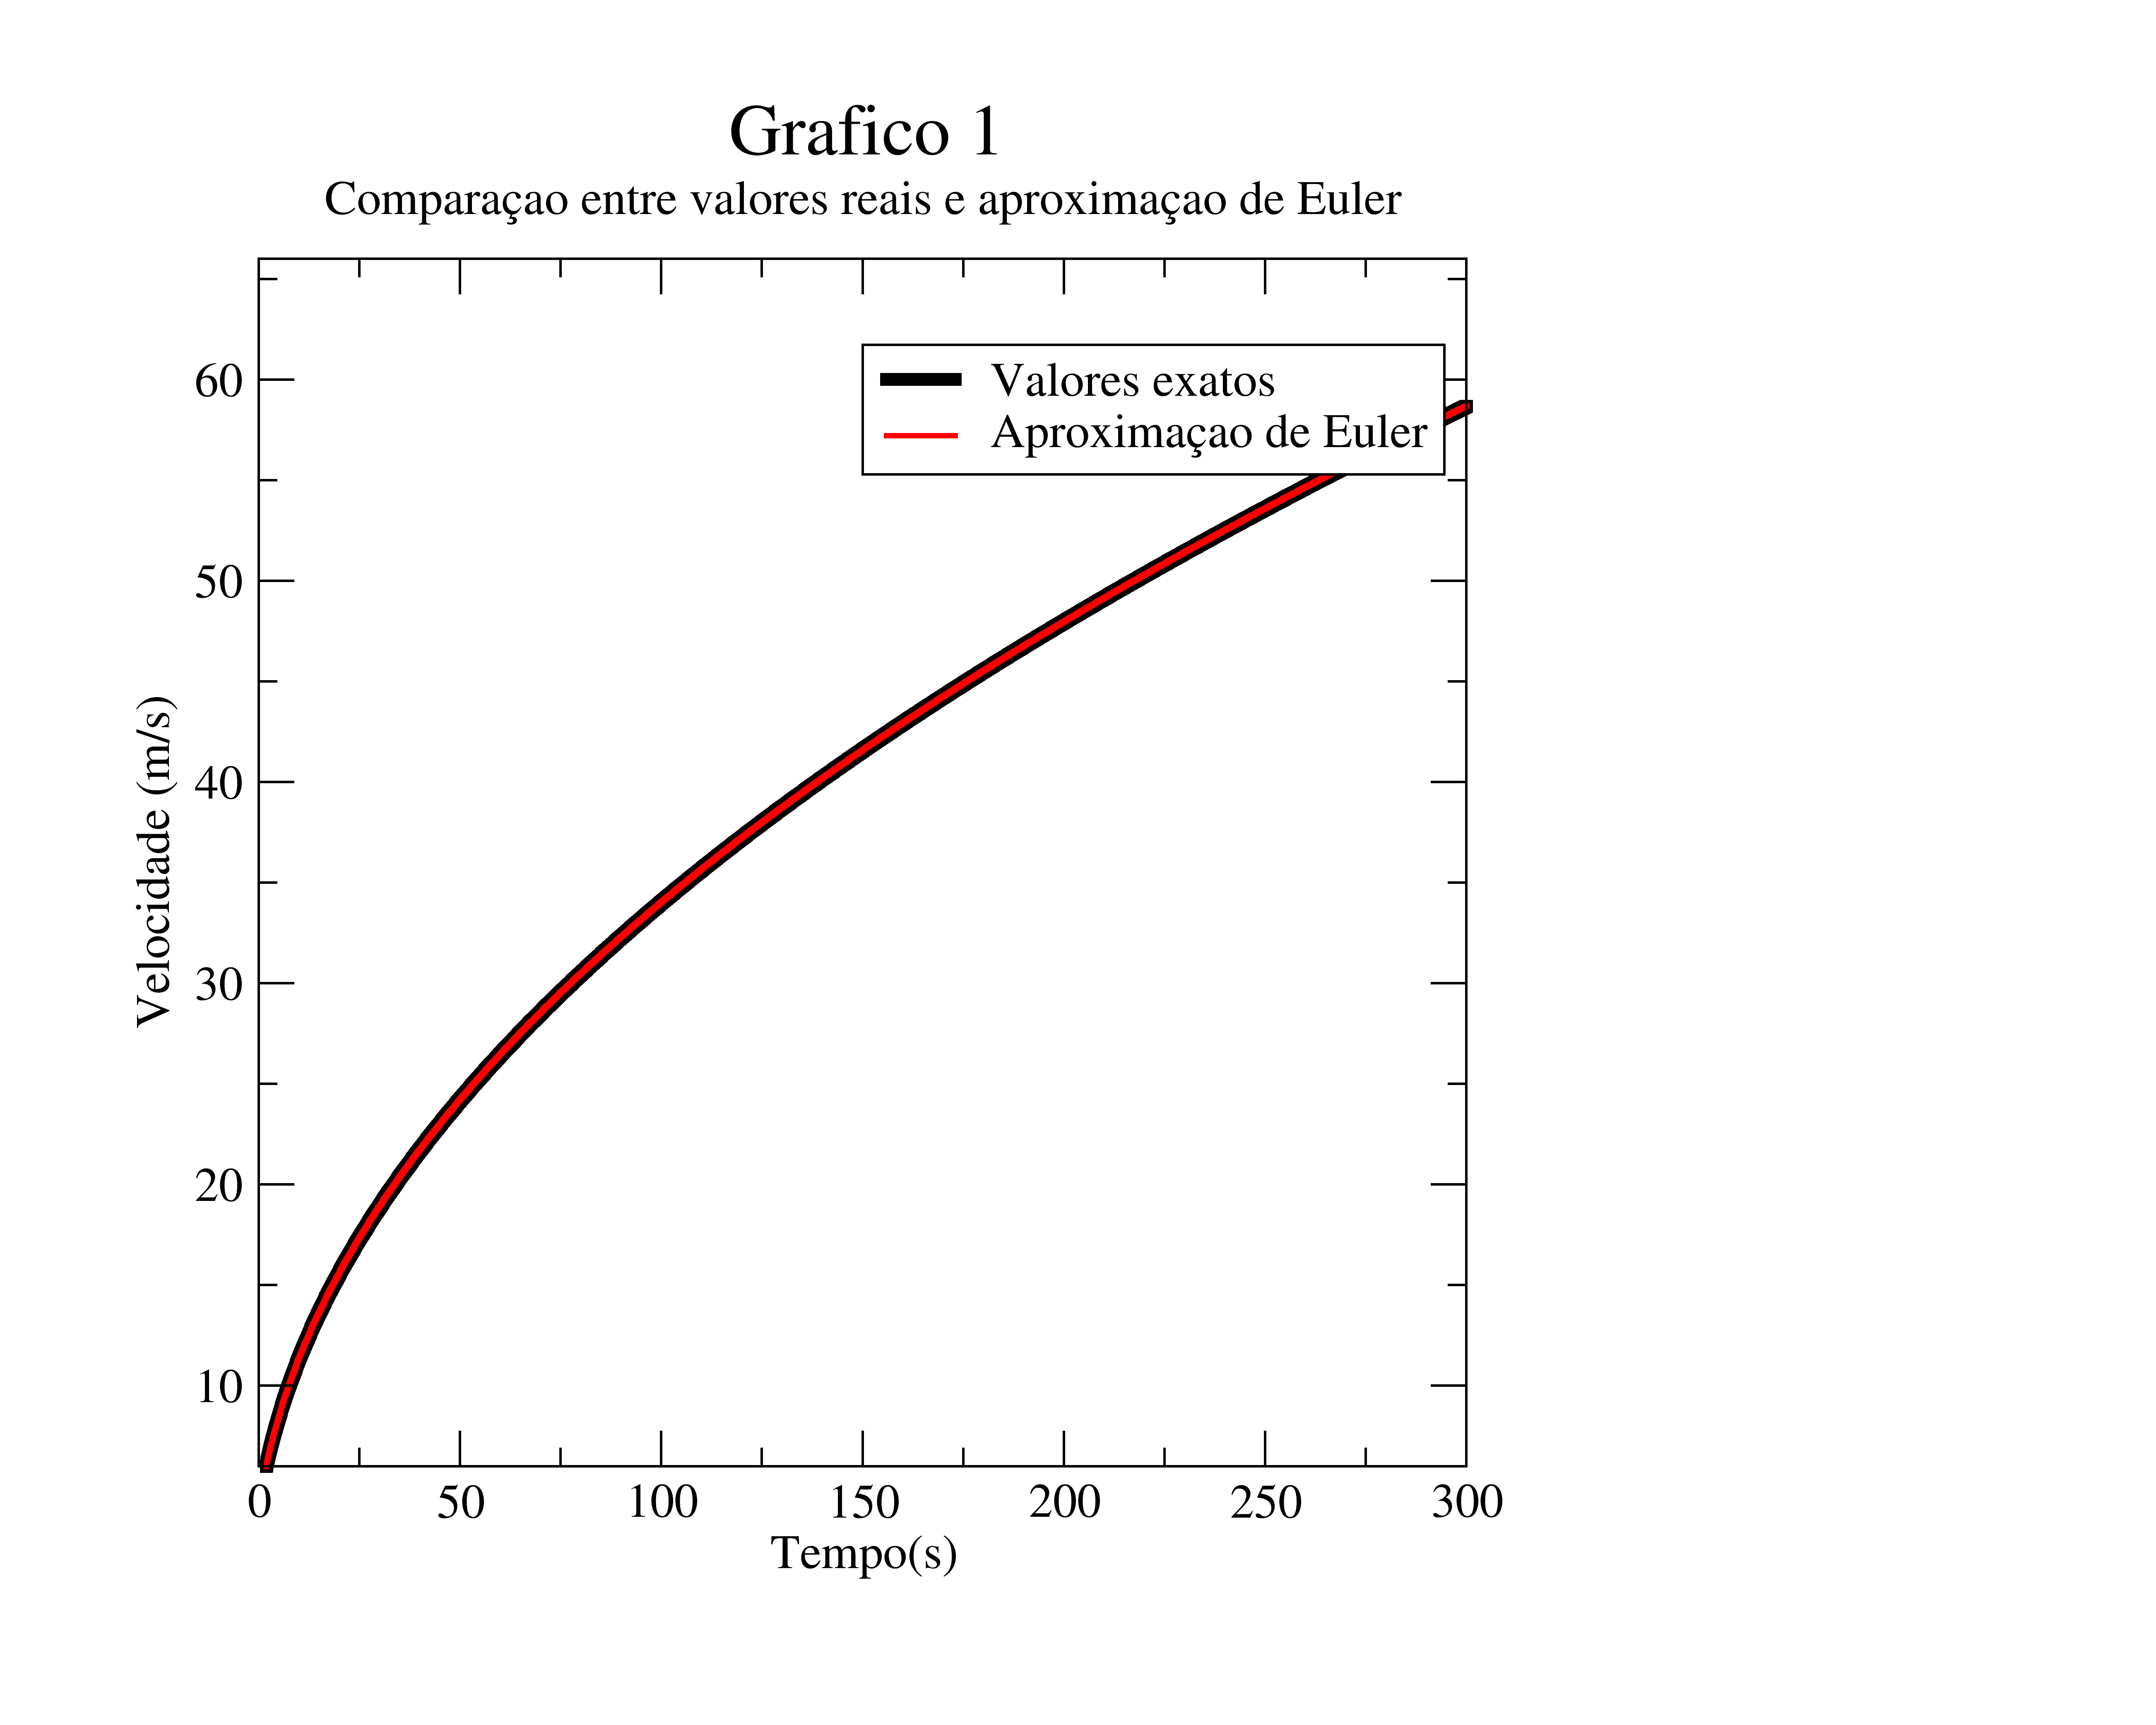
\includegraphics[width=.64\textwidth]{graf1}
\end{figure}

Pode se ver claramente que a velocidade não converge para um valor determinado, tende a um estado de crescimento linear com passar do tempo. Isto se deduz pela presença fortemente sugerida de assíntota oblíqua no gráfico 1.
%Deduzir equação da assíntota; Distância percorrida.

A seguir, foram fixados \(\rho = 1.3 kg m^{-3}\) e \(A= 0.333 m^2\) e o programa foi novamente utilizado, gerando valores que culminaram no gráfico 2.

\begin{figure}[h!]
  \centering
  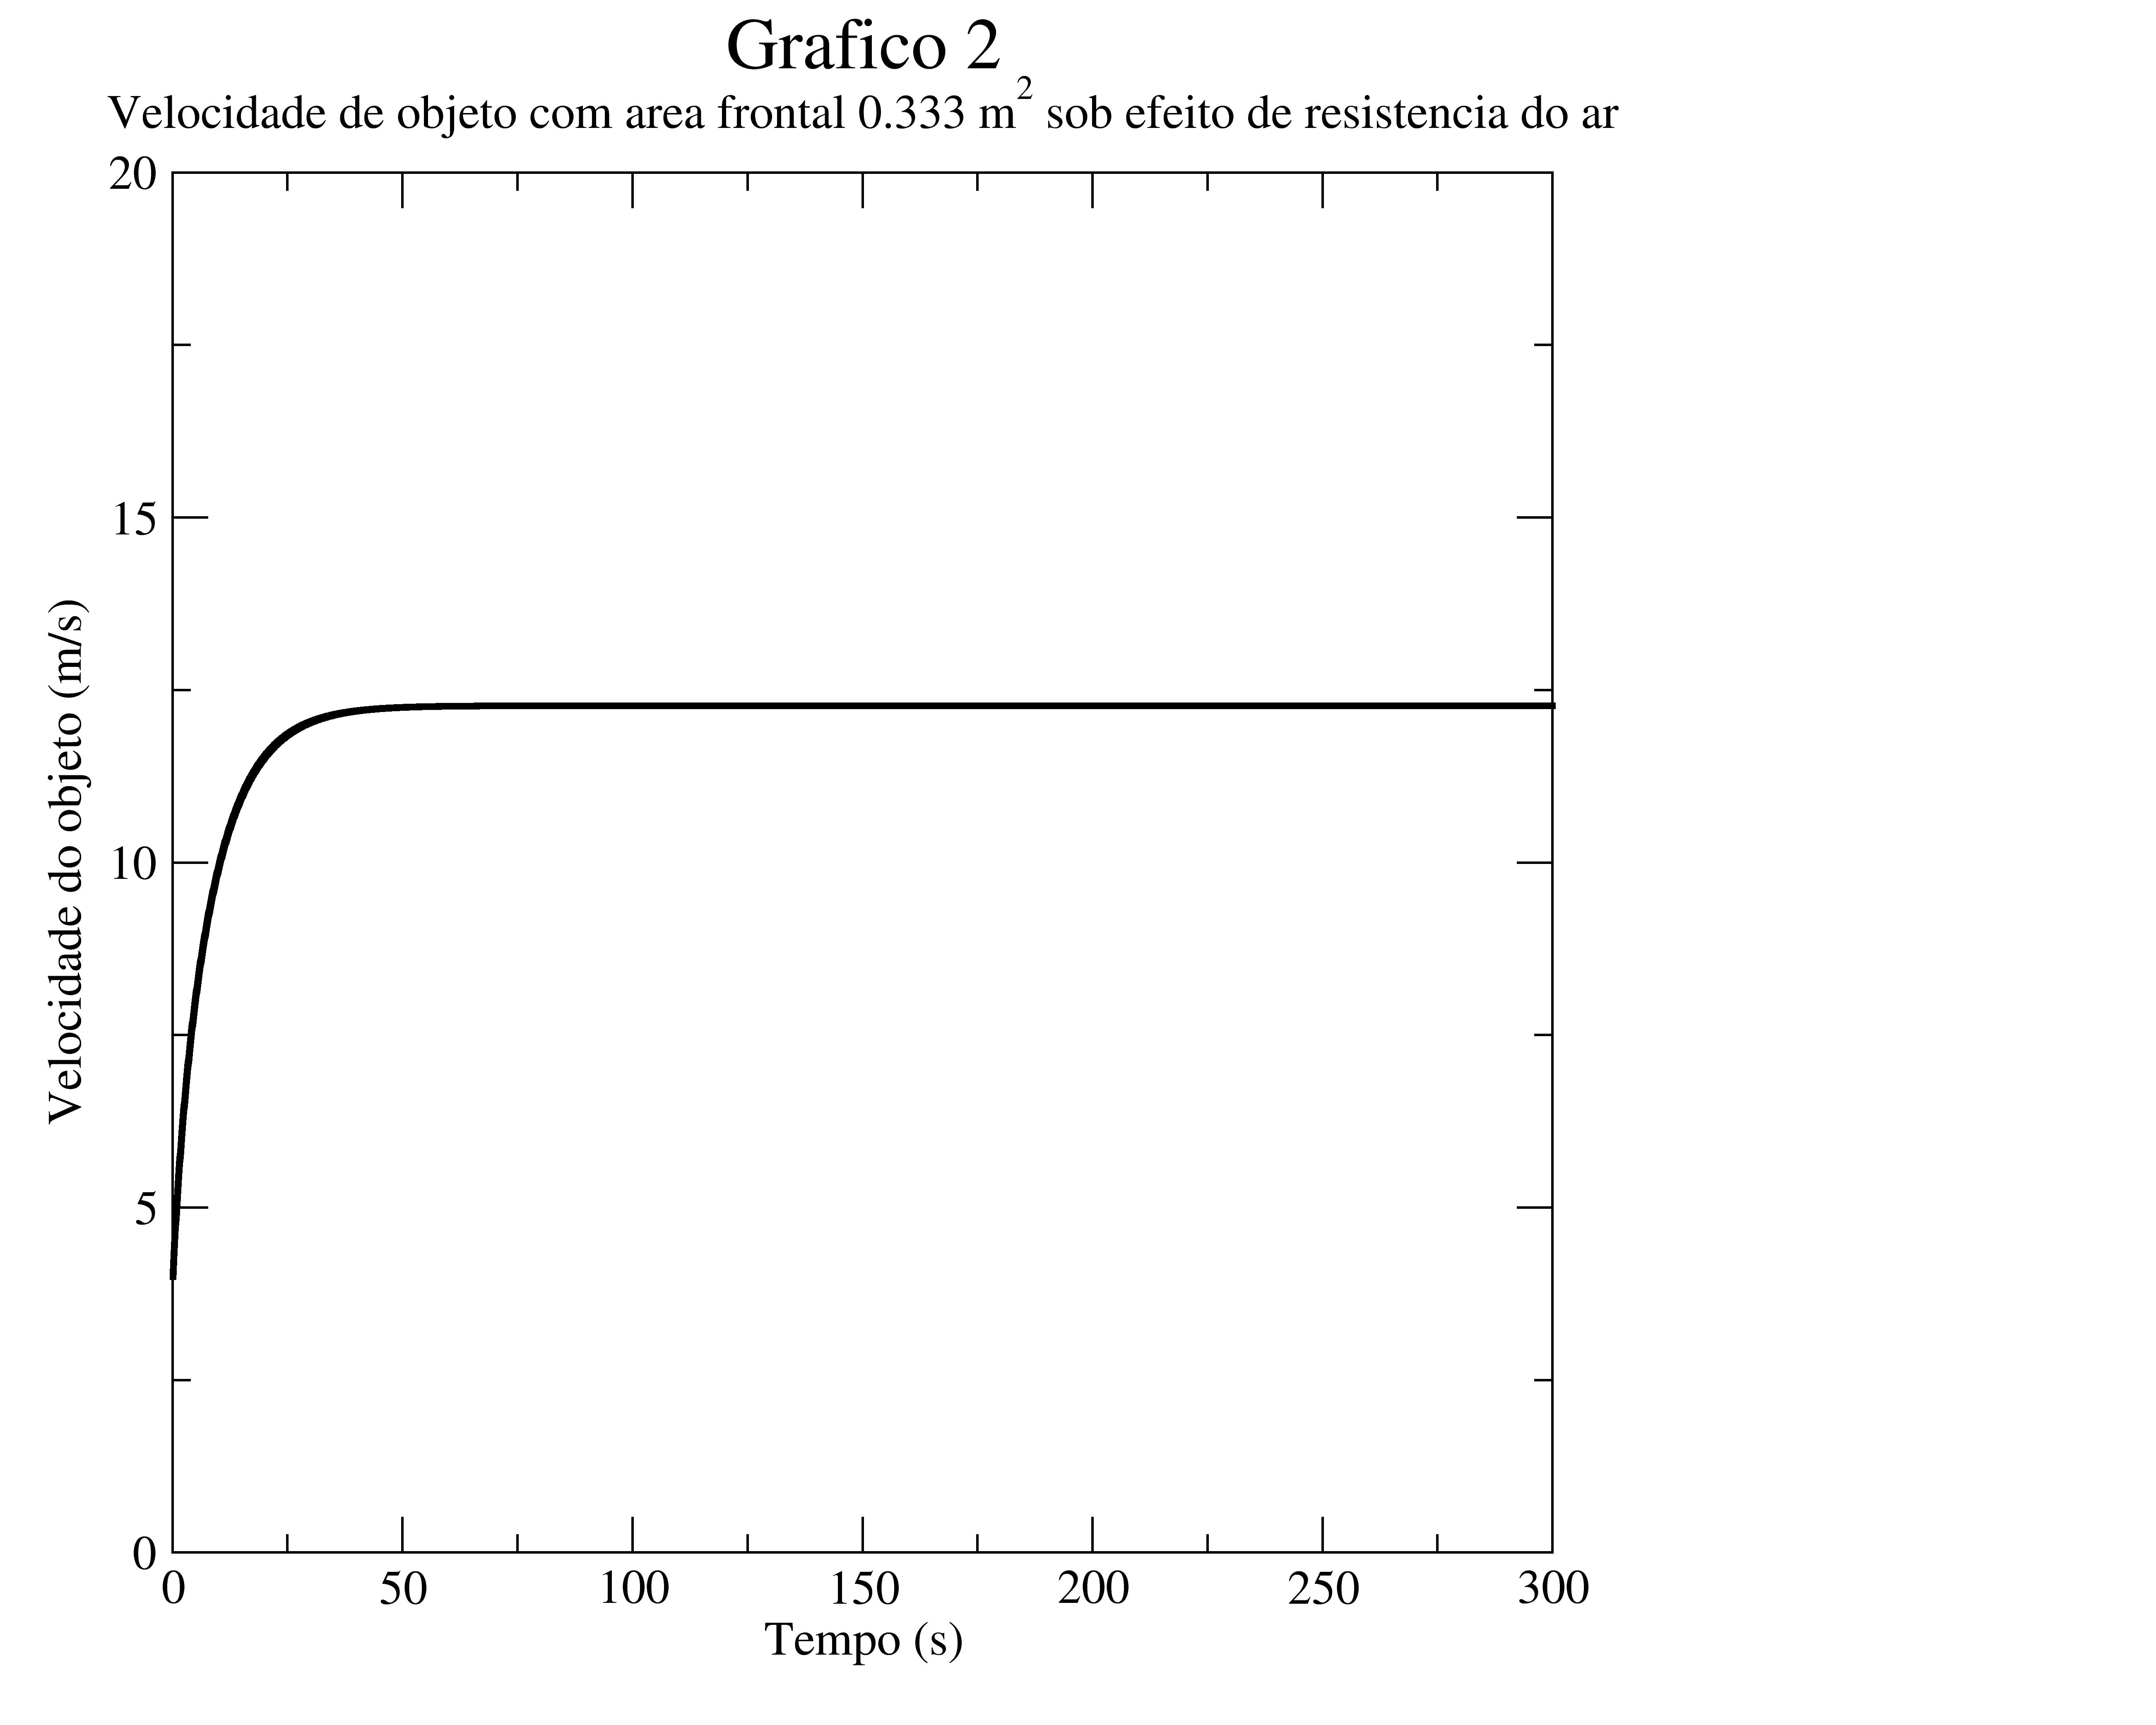
\includegraphics[width=.64\textwidth]{graf2}
\end{figure}

Os valores da velocidade retornados pelo programa convergiram, a partir do instante \(t=280.5s\), ao número 12.271589119894585, correspondente à velocidade terminal neste caso em m/s.\par
Utilizando a equação \ref{eq:3}, chega-se ao valor 12.271589119894672, que difere apenas a partir da décima terceira casa decimal em relação ao resultado do método aproximado.

\begin{equation}
  \label{eq:3}
  v_{terminal} = \left({2 P \over \rho A}\right)^{1\over3}
\end{equation}

A distância percorrida pelo ciclista no movimento representado pelos dois primeiros gráficos foi calculada com uso de FORTRAN, assumindo-se velocidade constante dentro de cada \(\Delta t\) e, portanto, somando-se \(v_i\Delta t\) de todos os intervalos de tempo considerados.\par
Disto resultam os valores (em m) 11797.044313018616 e 3616.1654669905975, de distância total percorrida para o caso sem resistência do ar (Gráfico 1) e com resistência (Gráfico 2), respectivamente.\par%discuta!!!
Foi realizado o mesmo procedimento de cálculo da evolução da velocidade para \(\rho = 1.3 kg m^{-3}\) e diversos valores de A. Disto resulta o gráfico 3.

\begin{figure}[h!]
  \centering
  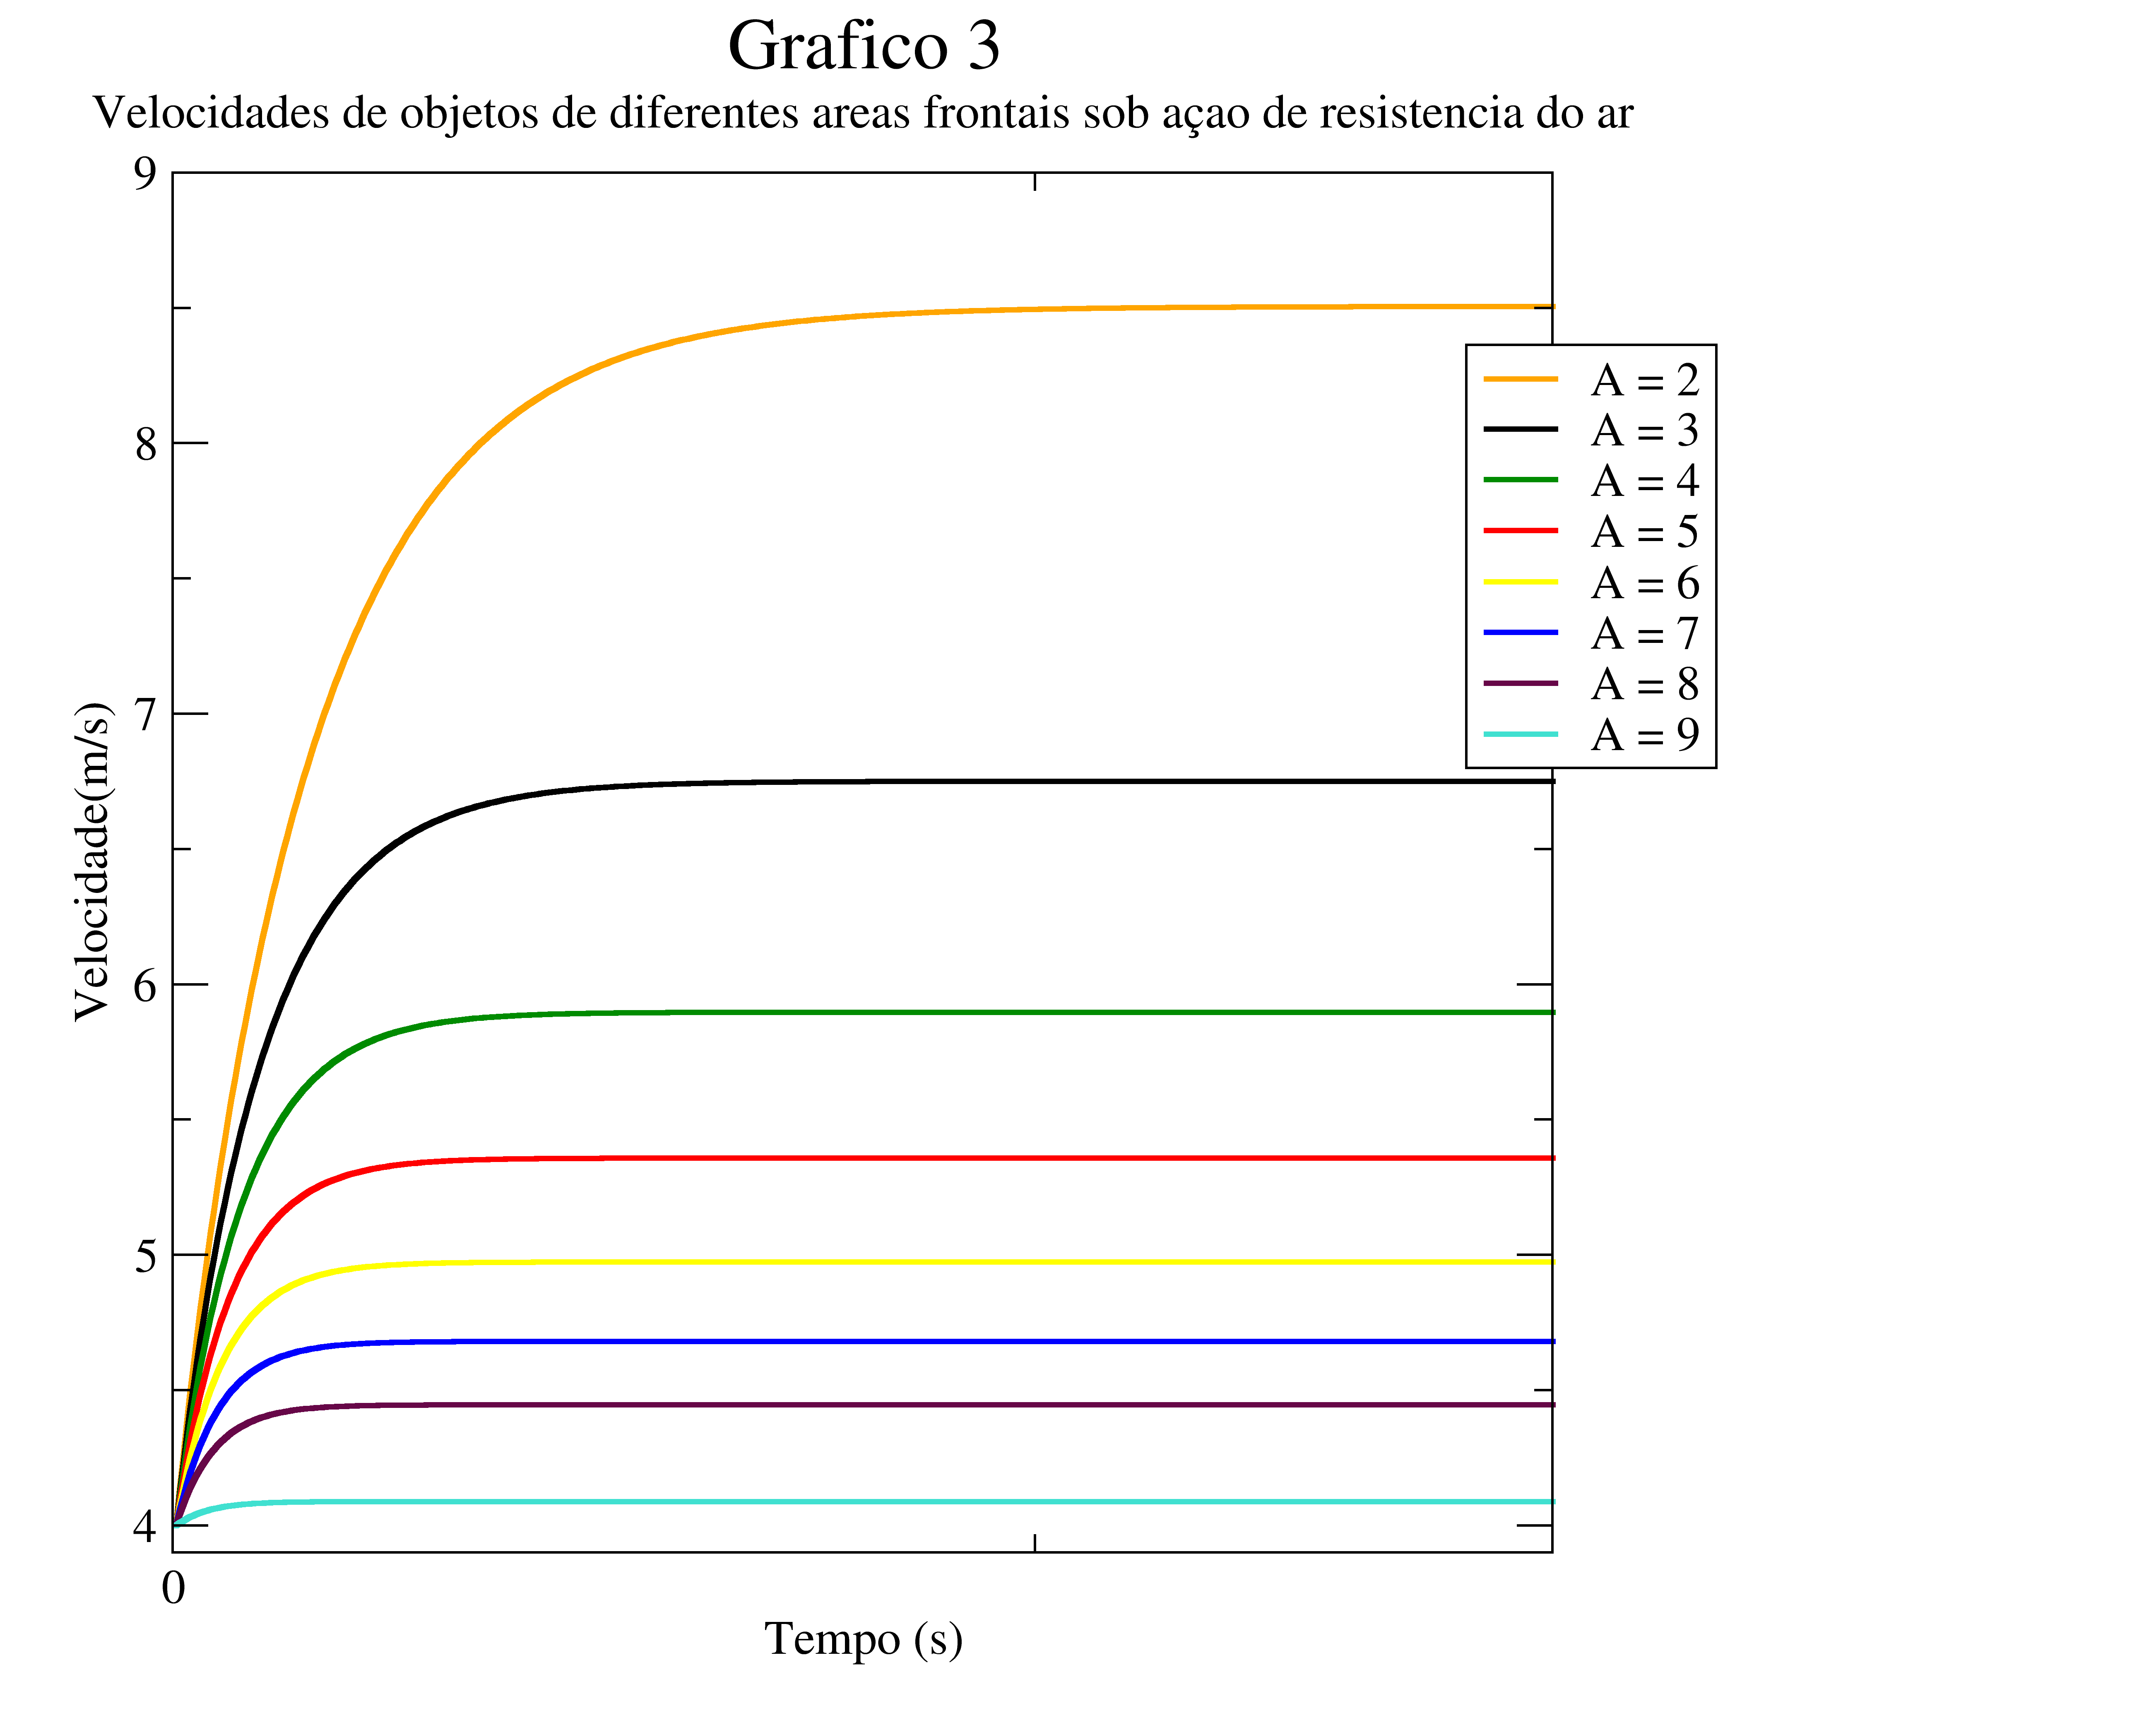
\includegraphics[width=.64\textwidth]{graf3}
\end{figure}

Pelo gráfico 3 deduzimos que as velocidades terminais são atingidas mais rapidamente e tem menor valor quanto maior for a área do objeto com velocidade sob efeito da resistência do ar.\par
No ciclismo profissional esse resultado é aproveitado com técnicas que visam minimizar a área frontal do ciclista e da bicicleta: o ciclistas se mantém o mais abaixados (com as costas na horizontal) que conseguem, e os pneus são feitos mais estreitos que os convencionais.

\newpage
\section{Lançamento de projéteis}

Nesta seção, foi desenvolvido um programa para simular a trajetória de um projétil lançado com velocidade inicial \(v_0 = 700ms^{-1}\) e ângulo \(\theta\) com a horizontal. Tal movimento é descrito pelas equações diferenciais:

\begin{equation}
  \label{eq:1}
  \begin{split}
  {d^2 x \over dt^2} = 0\\
\\
  {d^2y \over dt^2}= -g
\end{split}
\end{equation}
Em que $g = 9.80665$ é o valor adotado para a norma da aceleração da gravidade.
Da aplicação do método de Euler às equações \ref{eq:1} resulta o seguinte laço:

\begin{lstlisting}
  v=700
  vx=v*dcos(TETA)
  vy=v*dsin(TETA)

  DO WHILE (y .GE. 0)
        WRITE(10,*) x,y
        x = x + vx*dt
        y = y + vy*dt
        !vx=vx !vx constante
        vy = vy - g*dt
  END DO
\end{lstlisting}

Em que x e y são as respectivas posições horizontal e vertical, e vx e vy são as componentes horizontal e vertical da velocidade do projétil, definidas inicialmente em função de TETA = $\theta$.
Foram escritos oito arquivos de saída, para diferentes valores de TETA, que culminaram no gráfico 4.\par

\begin{figure}[h!]
  \centering
  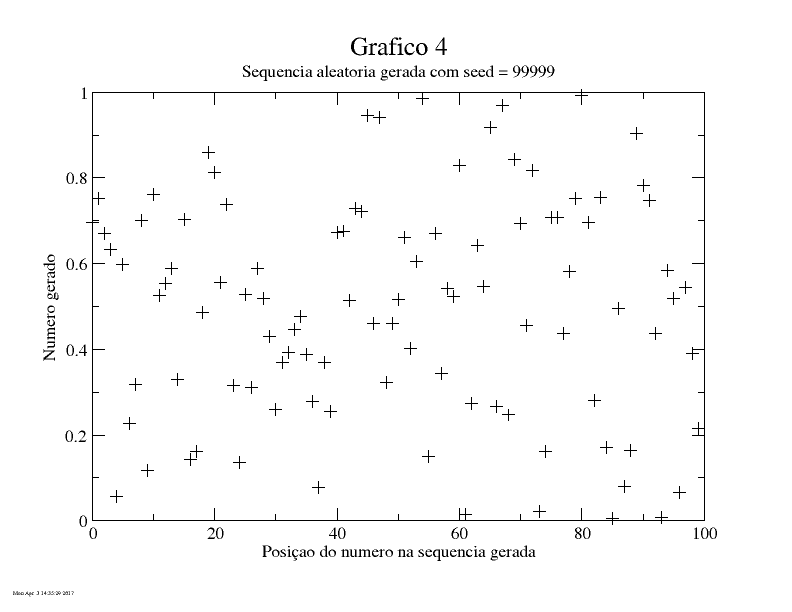
\includegraphics[width=.64\textwidth]{2/graf4}\par
\end{figure}


Observa-se que o maior deslocamento horizontal foi atingido com $\theta = 0.25 \pi$.\par
Da mesma forma que no caso anterior, estudar-se-á os efeitos da força de resistência do ar sobre as trajetórias, definida da seguinte forma:
\begin{equation}
  \label{eq:2}
  \vec{F}_{res} = -\gamma_2v\vec{v} = - \gamma_2 \sqrt{v_x^2 + v_y^2}\;\vec{v}
\end{equation}

De maneira a reformular, após aplicação do método de Euler, o laço escrito para o código a seguir:

\begin{lstlisting}
  DO WHILE (y .GE. 0)
        WRITE(10,*) x,y
        x = x + vx*dt
        y = y + vy*dt
        vx=vx - GAMA*v*vx*dt
        vy = vy - g*dt - GAMA*v*vy*dt
  END DO
\end{lstlisting}

No qual foi atribuído o valor $4\times 10^{-5}m^{-1}$ à constante GAMA, correspondende a $\gamma_2$ dividida pela massa do projétil. Disso resulta o gráfico 5.

\begin{figure}[h!]
  \centering
  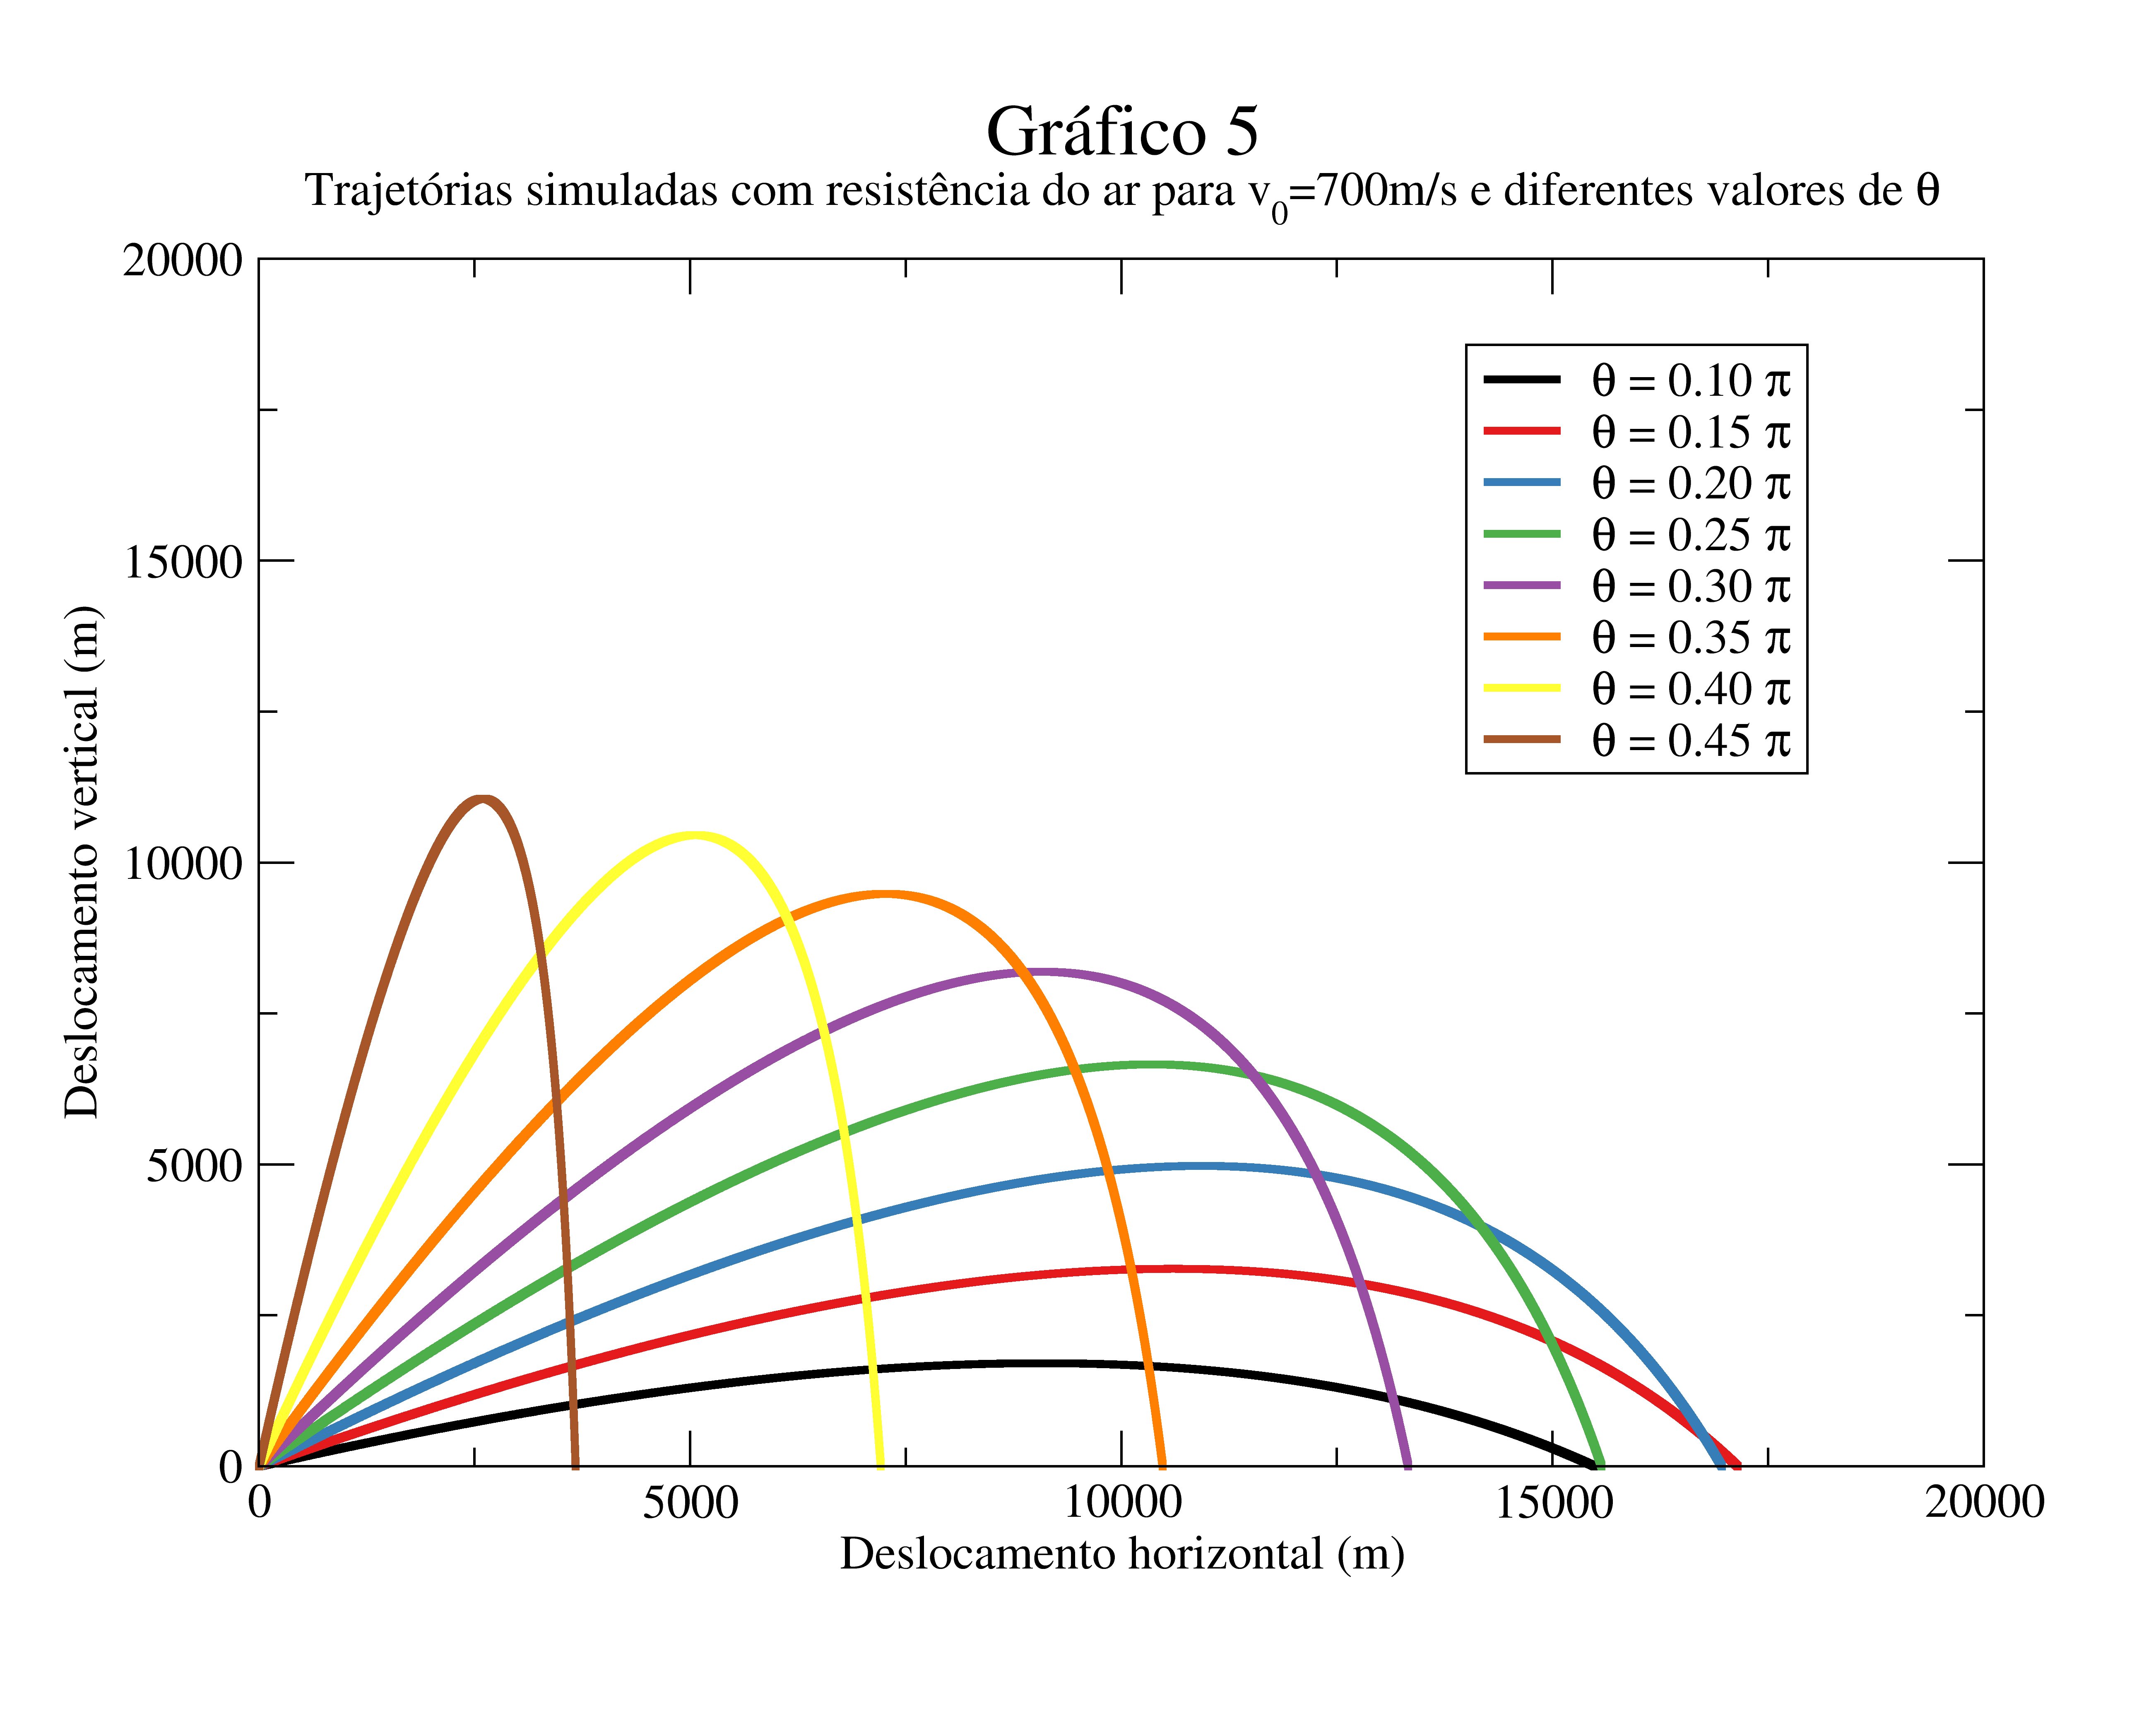
\includegraphics[width=.64\textwidth]{graf5}
\end{figure}

\par Neste caso, o ângulo de lançamento que gerou maior distância horizontal percorrida entre os casos estudados foi $0.15 \pi$.\par
Nota-se que as trajetórias de valor simétrico a $0.25 \pi$, que antes tinham mesmo alcance horizontal, perderam essa característica. Isto de deve à tendência de maior comprimento do trajeto de voo conforme mais vertical é a velocidade de início, o que permite maior trabalho da força de resistência e, portanto, mais perda de energia mecânica.
A seguir, plotou-se novamente as trajetórias dos lançamentos com $\theta=0.25\pi$ sob efeito e livre da força de resistência do ar (gráfico 6).

\begin{figure}[h!]
  \centering
  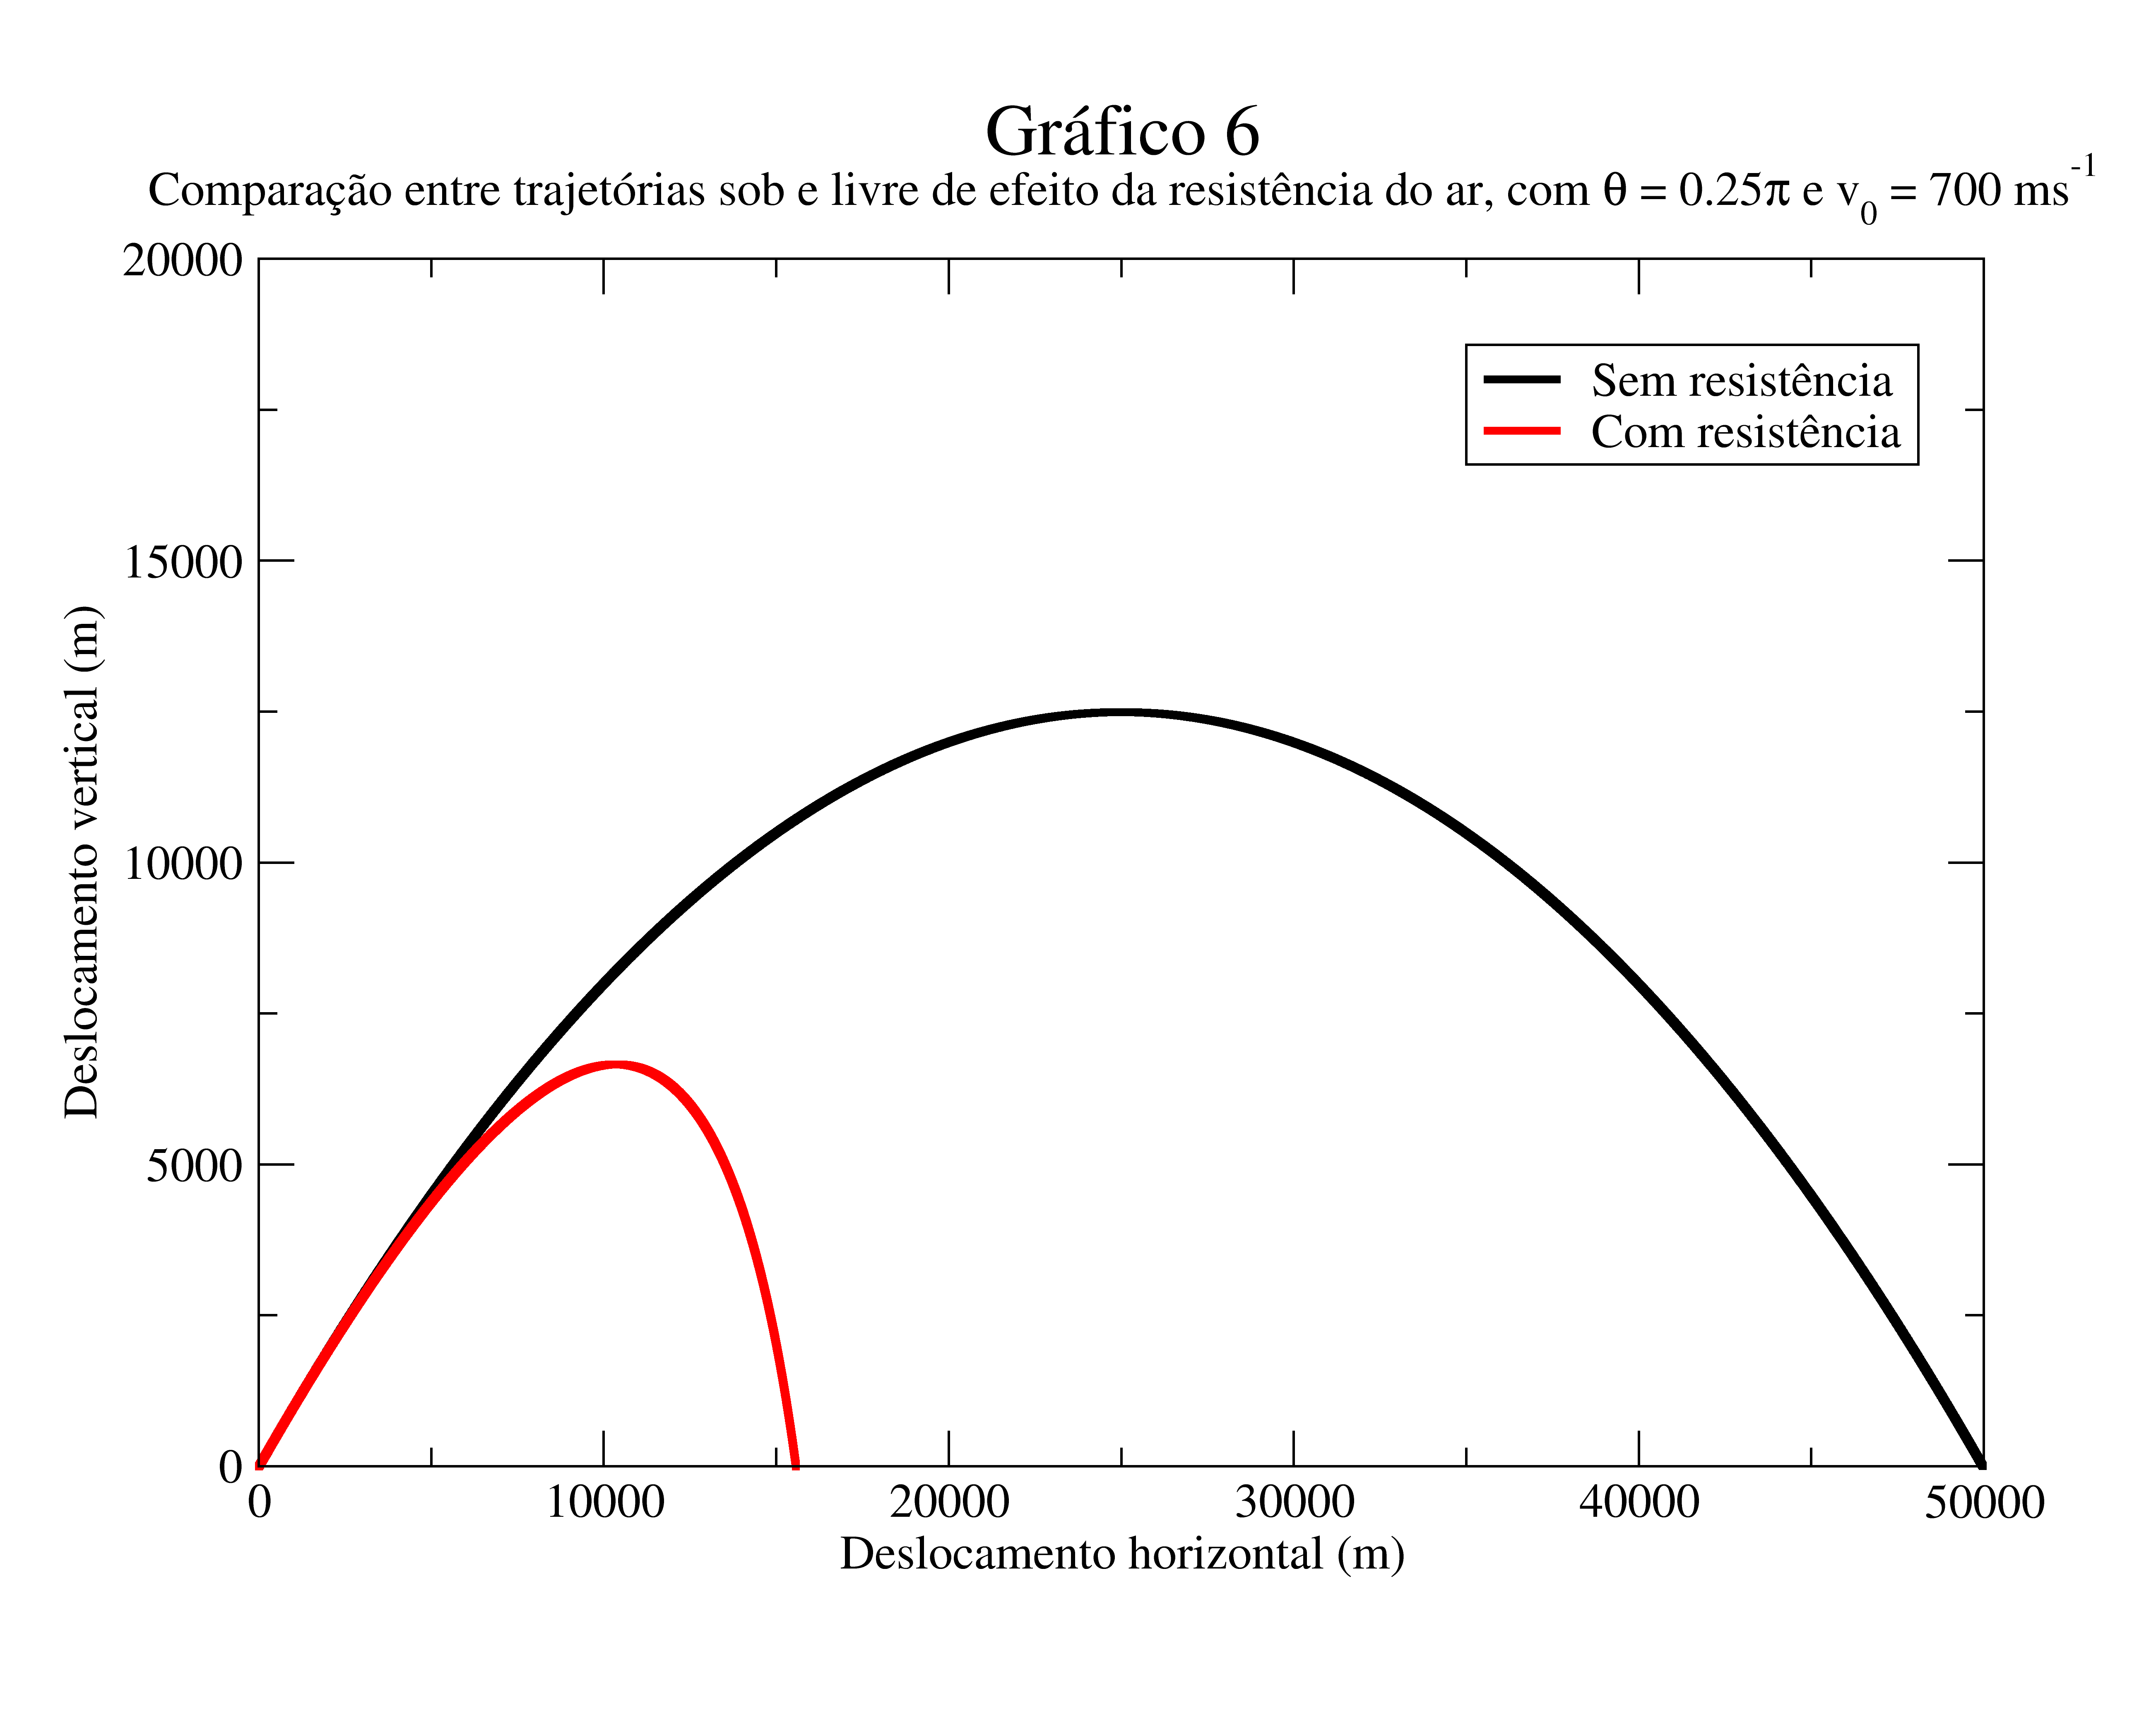
\includegraphics[width=.64\textwidth]{graf6.png}
\end{figure}

\par Fica clara a perda de energia mecânica decorrente da aplicação da força de resistência do ar, pois mesmo as velocidades iniciais, e portanto as energias cinéticas iniciais, dos projéteis sendo equivalentes, as alturas máximas atingidas, e portanto máximas energias potenciais gravitacionais, foram evidentemente diferentes.
\par Com efeito da resistência, infere-se também que a aproximação do trajeto por função quadrática deve perder precisão, dadas as distorções da órbita em relação ao caso sem resistência, sendo necessários outros meios de modelagem.

\newpage

\section{Pêndulo simples}
Estudar-se-á o movimento oscilatório de um pêndulo simples de comprimento $L$ e ângulo $\theta$ com a vertical, sob campo gravitacional g, representado pela equação a seguir.
\begin{equation}
  \label{eq:pendef}
  {d^2\theta \over dt^2} = -gL\sin{\theta}
\end{equation}
Cuja energia mecânica $E$ é dada pela equação \ref{eq:penen}.

\begin{equation}
  \label{eq:penen}
  E = frac{1}{2}mL^2\omega^2 + mgL(1 - cos{\theta})
\end{equation}
 
Onde $\omega = frac{d^2\theta}{d\theta^2}$.\par
A qual culmina, pelo método de Euler nas equações \ref{eq:peneuler}.

\begin{split}
  \begin{equation}
    \label{eq:peneuler}
    \omega_{i+1} = \omega_i-gL\sin{\theta_i}\Delta t
    \theta_{i+1} = \theta_i+\omega{1}\Delta t
\end{equation}

\end{split}
\par São estabelecidas as seguintes constantes:
\begin{itemize}
\item $L = 1 m$
\item $m=1kg$
\item $g = 10 ms_{-1}$
\item $\omega_0 = frac{\pi}{6}$
\end{itemize}

Assim, $E$, w = $\omega$ e TETA = $\theta$ são então calculados em laço:

\begin{lstlisting}
    TETA = PI/6.D0
    w = 0
    E = g*(1-DCOS(TETA))

    DO i=0, 20.D0/dt
        WRITE(10,*) i * dt, TETA
        WRITE(20,*) i * dt, E
        oldTETA = TETA
        TETA = TETA + w * dt
        w = w - g * DSIN(oldTETA) * dt
        E = .5D0 * w ** 2 + g * (1.D0-DCOS(TETA))
     END DO
\end{lstlisting}

Gerando os gráficos 7 e 8.

\begin{figure}
  \centering
  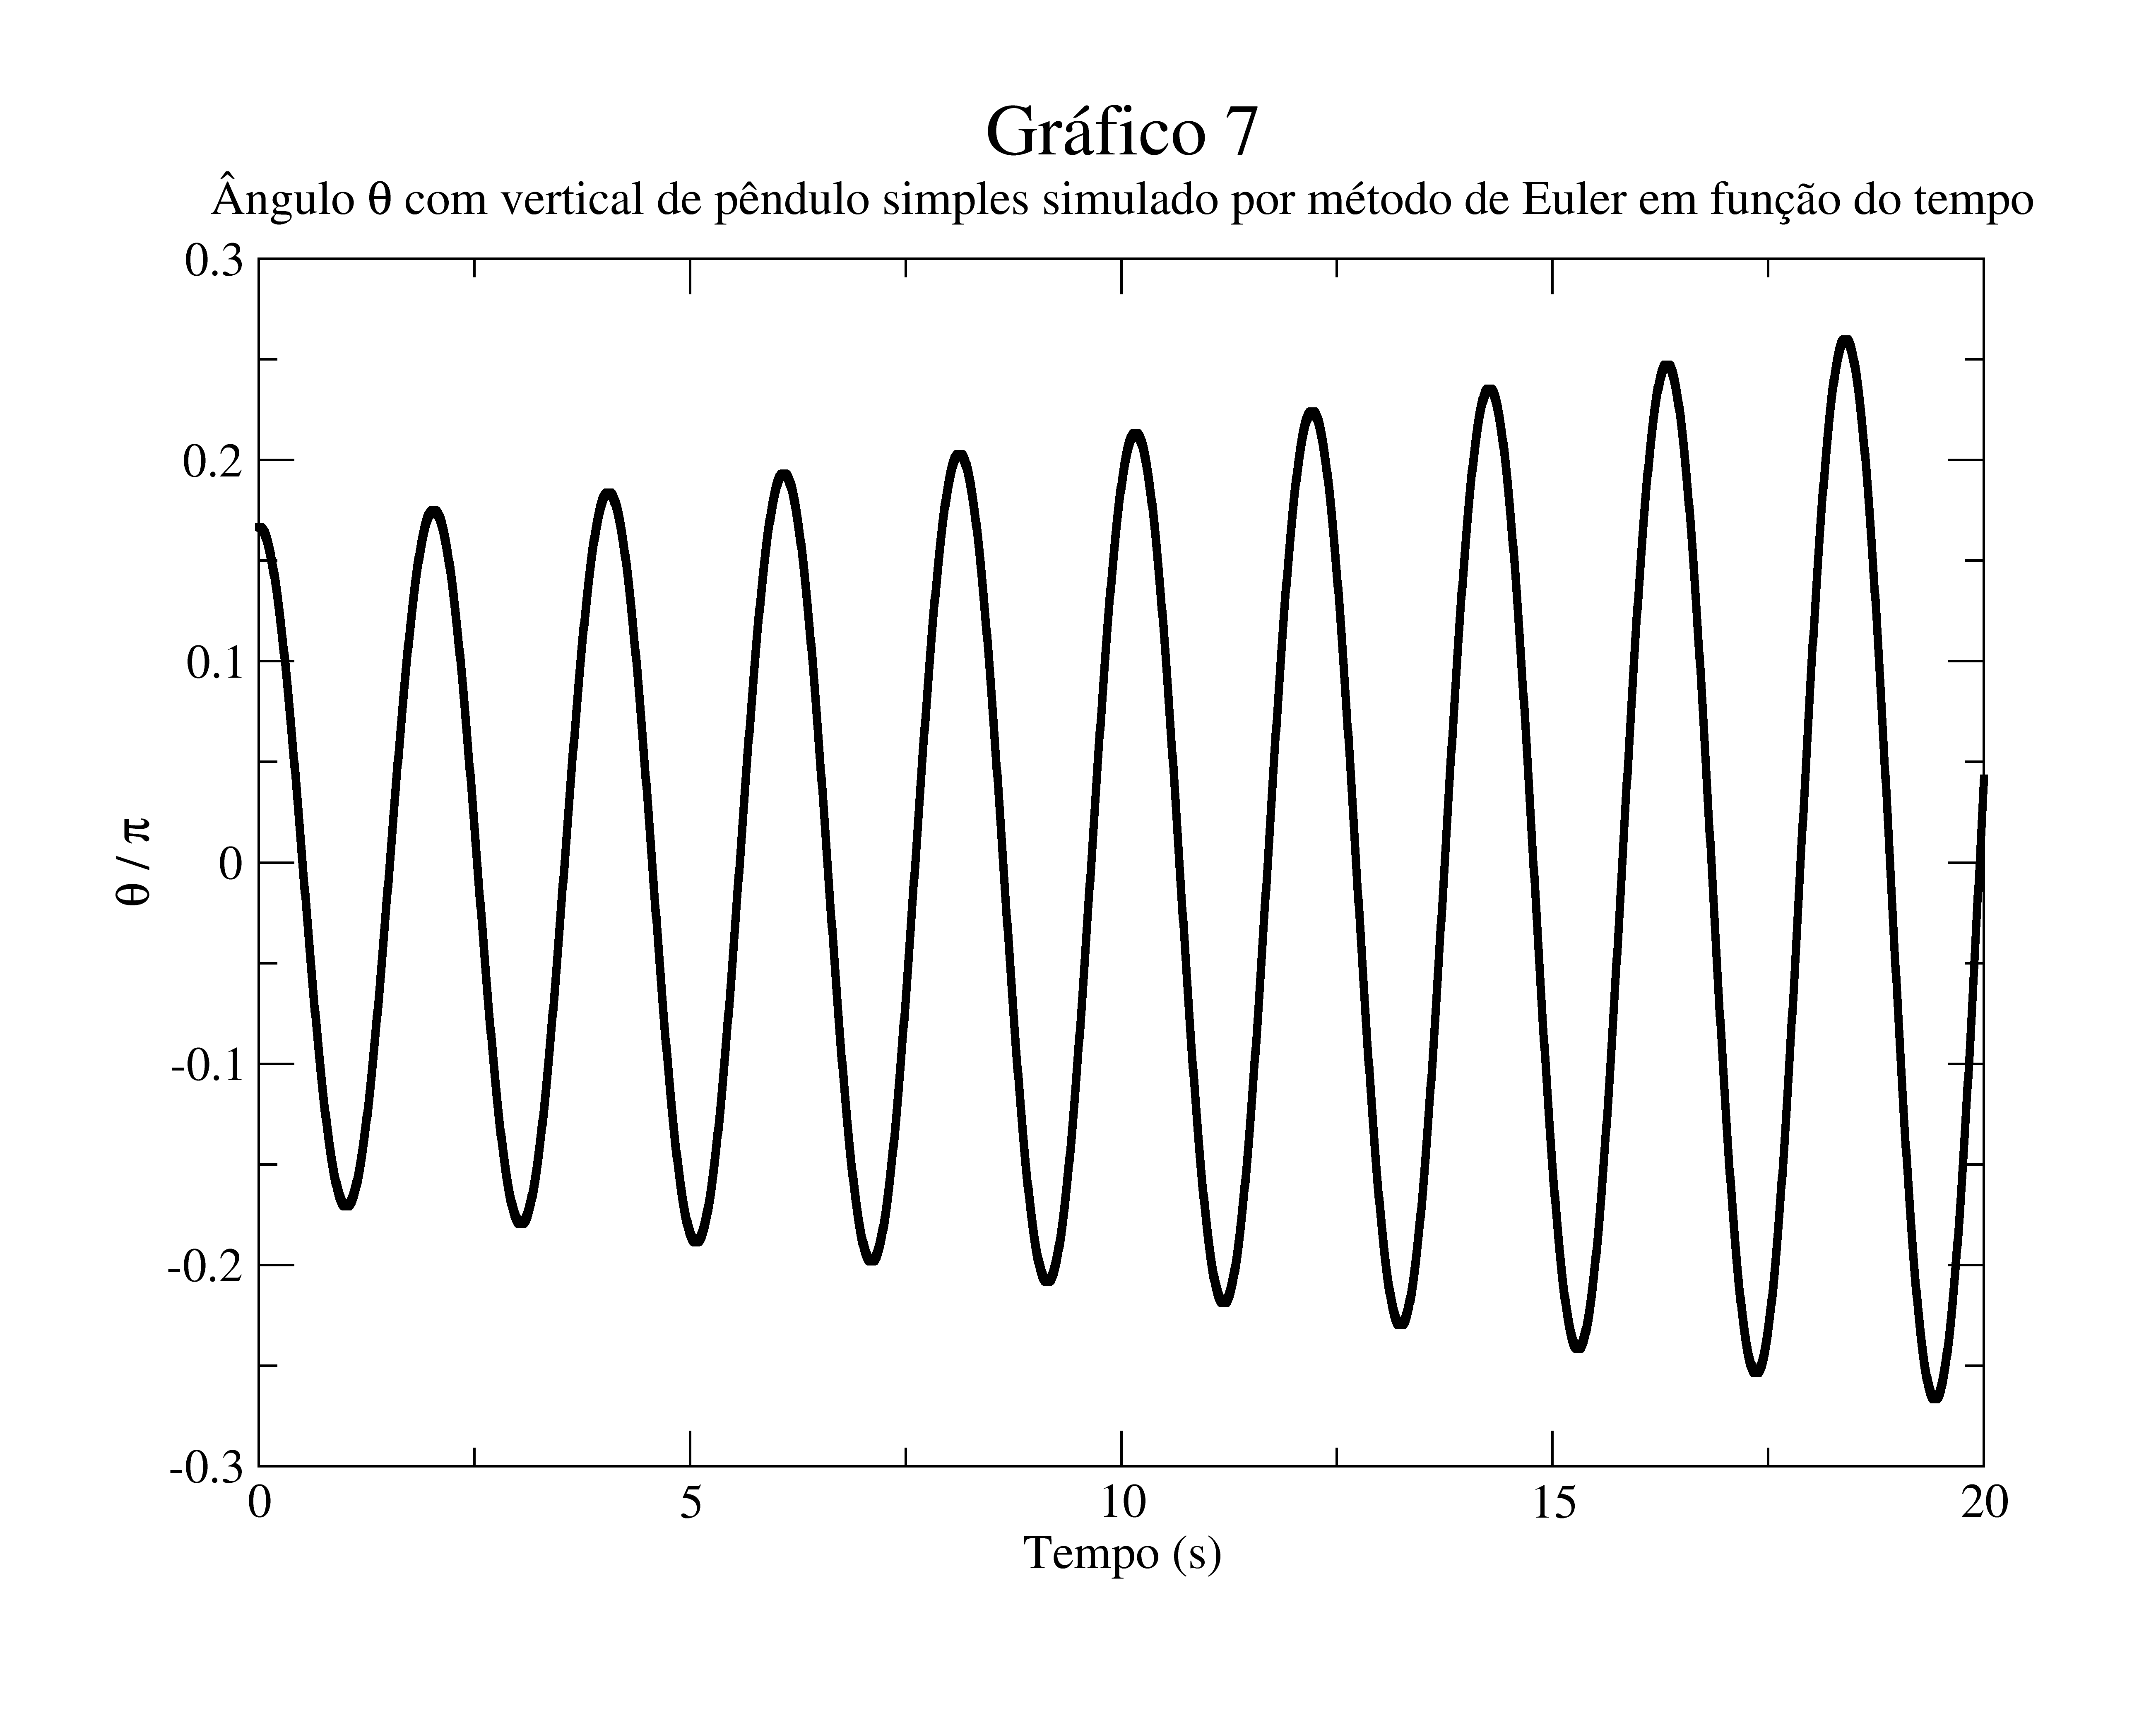
\includegraphics[width=.6\textwidth]{graf7.png}
\end{figure}

\begin{figure}
  \centering
  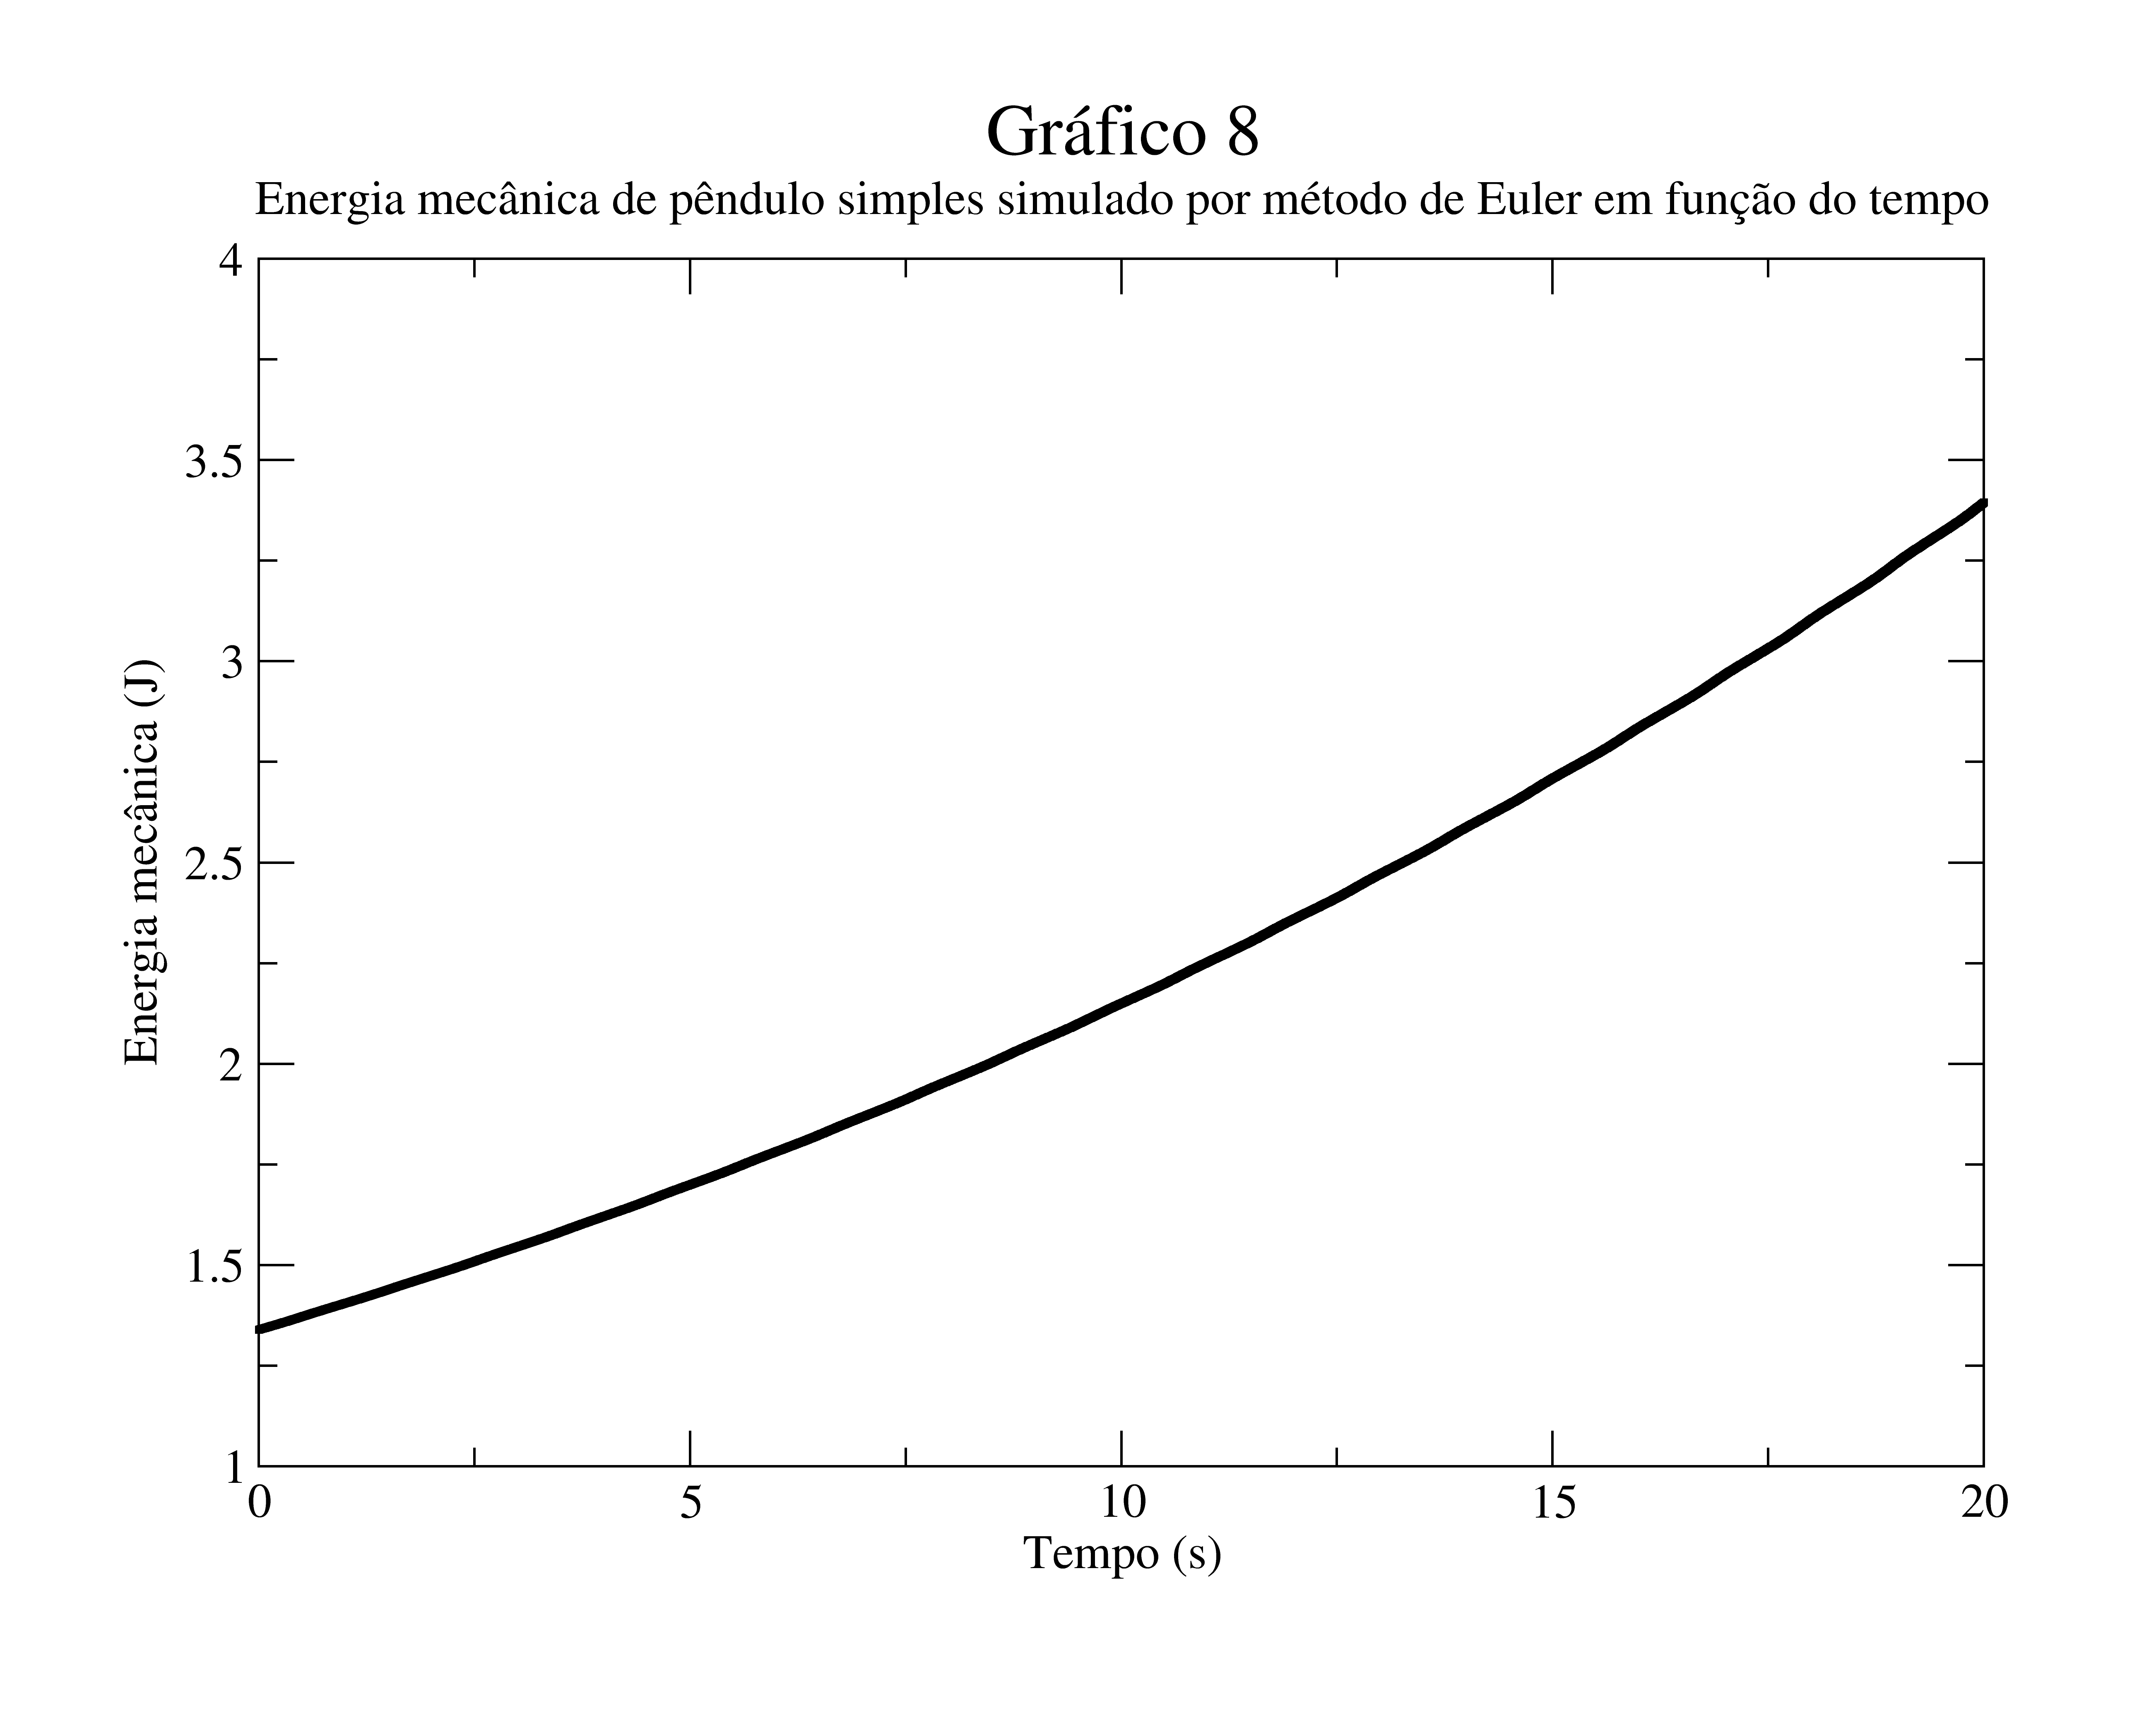
\includegraphics[width=.6\textwidth]{graf8.png}
\end{figure}


\end{document}
 